\documentclass[onecolumn]{IEEEtran}

\usepackage[left=1.5cm,right=1.5cm]{geometry}
\usepackage[
spanish,
es-nodecimaldot,
es-tabla
%english
]{babel}
\usepackage[utf8]{inputenc}
\usepackage[T1]{fontenc}
\usepackage{float}
\usepackage{crossreftools}
\usepackage{graphicx}
\usepackage{grffile}
\usepackage{longtable}
\usepackage{wrapfig}
\usepackage{rotating}
\usepackage[normalem]{ulem}
\usepackage{amsmath}
\usepackage{textcomp}
\usepackage{amssymb}
\usepackage{capt-of}
\usepackage{hyperref}
\usepackage{minted}
\usepackage{subfiles}
\usepackage{caption}
\usepackage{subcaption}
\usepackage[acronym, toc]{glossaries}


\usepackage{fancyhdr}
\usepackage{graphicx}
\usepackage[table,xcdraw]{xcolor}
\usepackage{multicol}
\usepackage{tabularx,booktabs}
\usepackage{siunitx}

\usepackage{grffile}
\usepackage{longtable}
\usepackage{rotating}
\usepackage[normalem]{ulem}
\usepackage{amsmath}
\usepackage{textcomp}
\usepackage{amssymb}
\usepackage{capt-of}
\usepackage{booktabs}
\usepackage{hyperref}
\usepackage{caption}

\definecolor{LightGray}{gray}{0.9}
\definecolor{DarkGray}{HTML}{191919}
\definecolor{custom}{HTML}{F8F8F8}

\newenvironment{code}{\captionsetup{type=listing}}{}

\usemintedstyle{emacs}

\usepackage[ruled,vlined]{algorithm2e}


\renewcommand{\listingscaption}{Código}
\renewcommand\listoflistingscaption{Índice de \listingscaption\@s}

\setminted[python]{frame=single,framesep=3mm,baselinestretch=0.9,breaklines=true,bgcolor=custom,fontsize=\scriptsize,linenos}
\setminted[shell-session]{frame=single,framesep=1mm,baselinestretch=0.5,breaklines=true,bgcolor=custom,fontsize=\scriptsize}
\graphicspath{
  {./img_common}
  {./img}
}
% \usepackage[T1]{fontenc}
% \renewcommand*\familydefault{\sfdefault} %% Only if the base font of the document is to be sans serif

% \pagestyle{fancy}
% \fancyfoot[R]{\thepage}
% \fancyfoot[C]{\includegraphics[width=0.05\textwidth]{inge_logo}}
% \fancyhead[L]{\leftmark}
% \fancyhead[R]{\rightmark}


\usepackage{authblk}
\usepackage[backend=biber,style=ieee]{biblatex}
\addbibresource{./main.bib}

\begin{document}

\begin{titlepage}
  \centering
  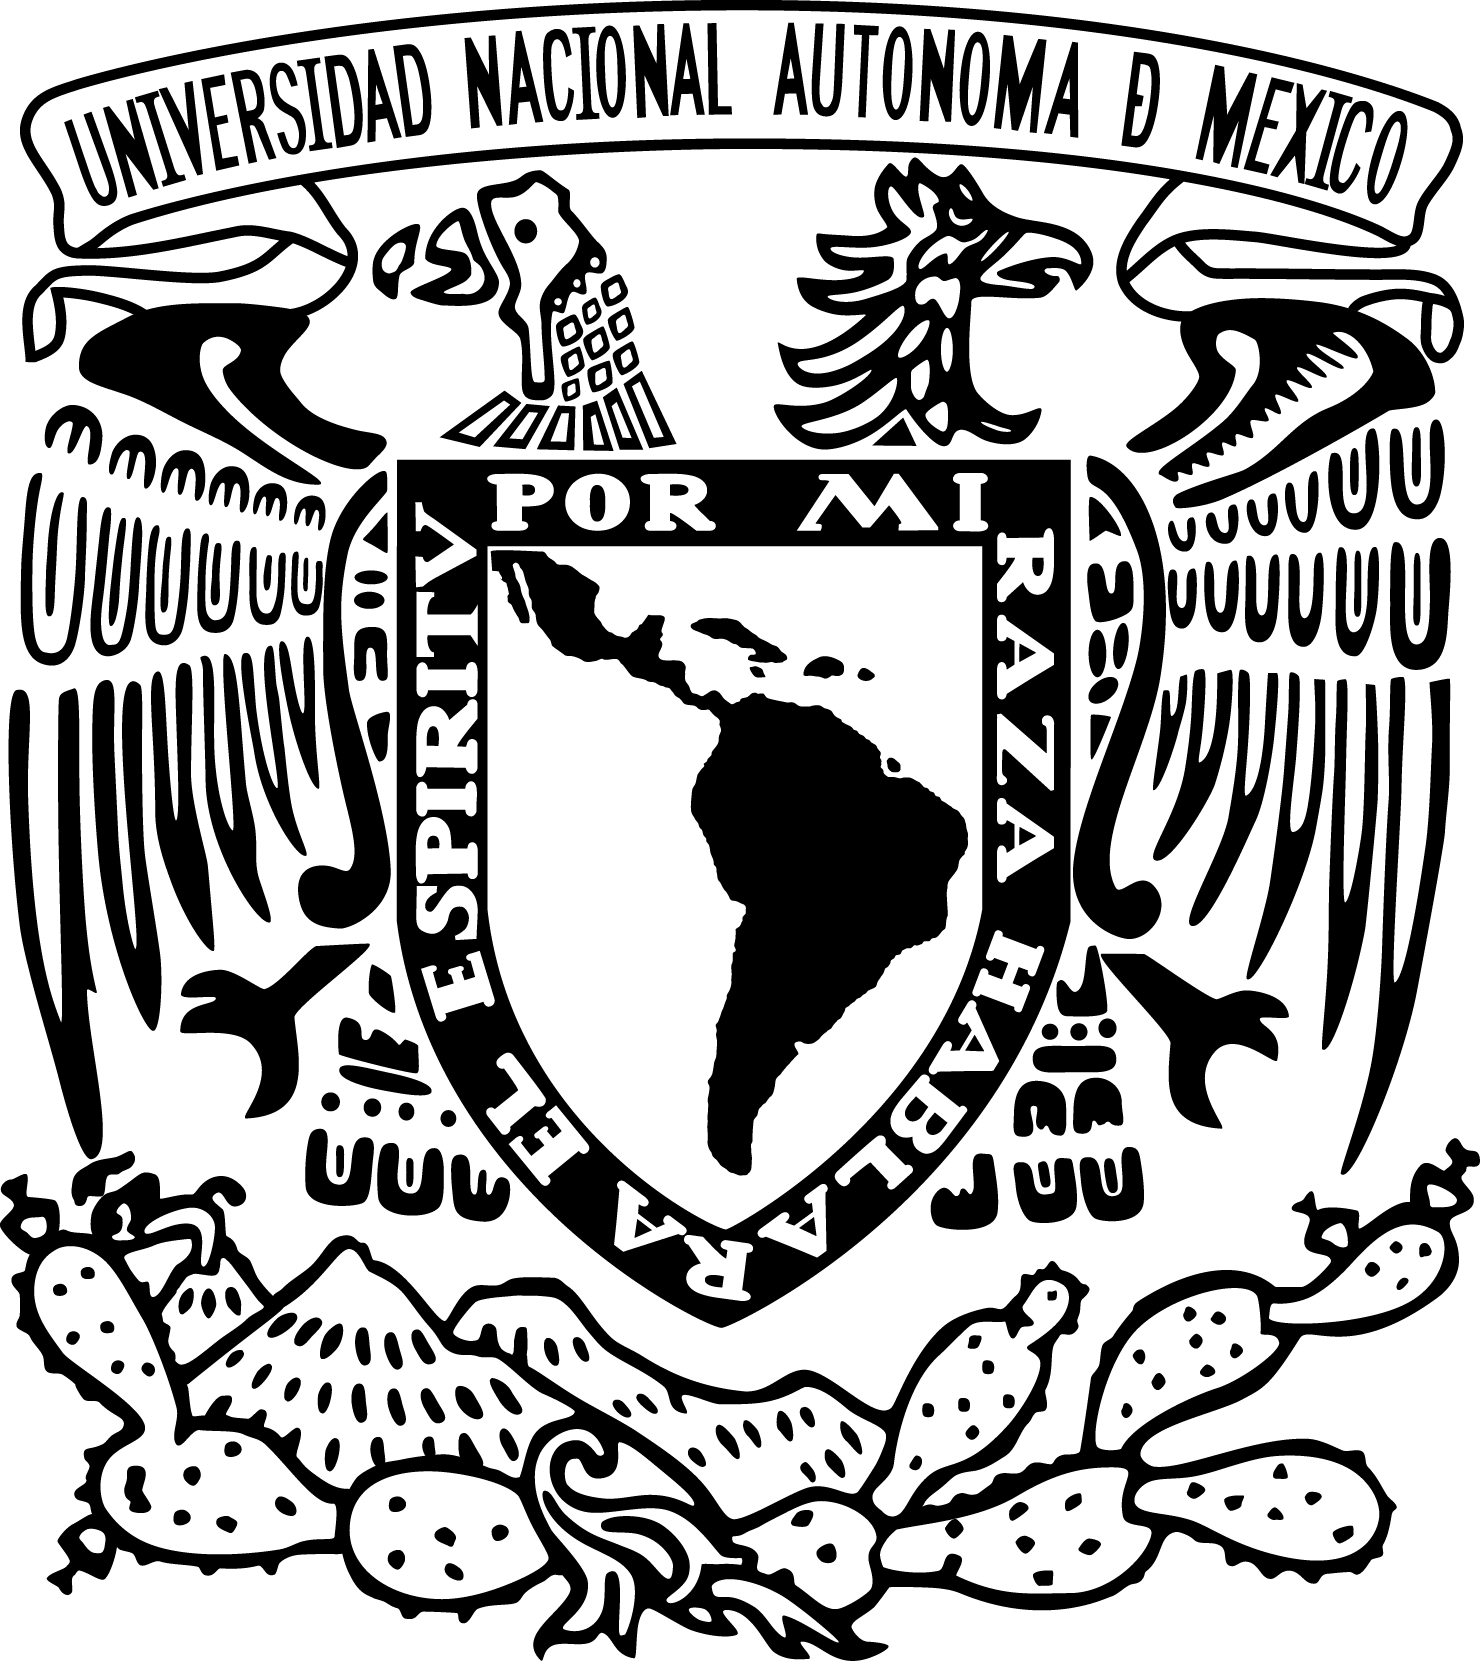
\includegraphics[width=0.3\textwidth]{unam-escudo}\vfill{}
  \Huge{Facultad de Ingeniería}\\
  \huge{Criptografía}\vfill{}
  \Huge{Proyecto Final}
  \\
  \vfill{}
  \LARGE{Alumnos:}
  \begin{flushleft}
    \begin{itemize}
      \item Machicao Cardoso Raúl Fernando
      \item Martínez López Andrés
      \item Romero Andrade Cristian
      \item Romero Andrade Vicente
    \end{itemize}
  \end{flushleft}
  \vfill{}
  % \Large{Grupo: 6}\\
  \Large{Semestre 2021--2}
  \vfill{}
  \LARGE{Profesora: Dra.~Rocio Alejandra Aldeco Perez}
  \vfill
  % \Large{Fecha de entrega: 14 de junio de 2021}
  % \vfill
  
\includegraphics[width=0.1\textwidth]{fi_logo}
\end{titlepage}


\title{Proyecto Final}
\author{
  \IEEEauthorblockN{
    Romero Andrade Cristian\IEEEauthorrefmark{1},
    Romero Andrade Vicente\IEEEauthorrefmark{2},
    Machicao Cardoso Raúl Fernando\IEEEauthorrefmark{3} y
    Martínez López Andrés\IEEEauthorrefmark{4}
  }
  \IEEEauthorblockA{Criptografía,
    Facultad de Ingeniería\\
    Email: \IEEEauthorrefmark{1}\href{mailto:cristian.romero@comunidad.unam.mx}{cristian.romero@comunidad.unam.mx},
    \IEEEauthorrefmark{2}\href{mailto:dark_reggae_93@comunidad.unam.mx}{dark\_reggae\_93@comunidad.unam.mx},
    \IEEEauthorrefmark{3}\href{mailto:laastar@comunidad.unam.mx}{laastar@comunidad.unam.mx},
    \IEEEauthorrefmark{4}\href{mailto:bockerlaila@comunidad.unam.mx}{bockerlaila@comunidad.unam.mx}}}

\maketitle{}

\tableofcontents{}

\begin{abstract}
    Para el presente trabajo comparamos varios algoritmos desde AES, pasando por SHA hasta las de curva elíptica como ECDSA, cada uno para una o unas tareas específicas. En principio al entender que cada uno de estos algoritmos se enfocan en diferentes objetivos los cuales podemos definir en tres métodos principales como Cifrado y descifrado (sección~\ref{sec:cifrado-y-descifrado}), Hashing (sección~\ref{sec:hash}) y Firma y Verificación (sección~\ref{sec:firma-y-verificacion}), es como podemos entender y realizar las pruebas necesarias para evaluar que tan eficaces son dichos algoritmos.
\end{abstract}

\subfile{./secciones/introduccion.tex}

\newpage{}

\subfile{./secciones/desarrollo.tex}

\clearpage{}

\section{Conclusiones}\label{sec:concluciones}

Una vez analizado los diferentes algoritmos en este trabajo, podemos decir que, si bien algunos de estos algoritmos destacan en su velocidad, no cabe duda que pueden llegar a sacrificar robustez (tal como pasó con SHA–1 en su momento). Unos algoritmos son más nuevos que otros, por lo cual los más recientes tienen ciertos antecedentes que benefician para su diseño teniendo una excelente relación velocidad—seguridad.

En conclusión, los diversos tipos de algoritmos ofrecen diferentes características las cuales dependiendo de lo que busquemos, ya sea mayor velocidad, mayor seguridad, mayor veracidad, etc. Es como debemos elegirlos y aplicarlos, ya que debemos buscar lo que nos de mayor eficiencia posible sin arriesgar tanto, es por eso que como se observó en el presente trabajo, para cada tipo de archivo que nosotros encriptemos o firmemos corresponderá al tiempo en el que se descifra o verifica el archivo, de esta forma con las pruebas realizadas y con los diferentes parámetros con los que se probaron los algoritmos AES, RSA, SHA-2, SHA-3, DSA y ECDSA es como podemos optar por un método de encriptación que nos garantice la autenticidad de nuestros archivos.
\nocite{*}

\newpage{}

\section*{Anexos}
\addcontentsline{toc}{section}{Anexos}

\listoffigures{}
\listoftables{}
\listoflistings{}
\bigskip{}
\faGithub~\href{https://github.com/ValdrST/test_algoritmos_crypto}{Enlace al repositorio}
\dotfill
\href{https://github.com/ValdrST/test_algoritmos_crypto}{https://github.com/ValdrST/test\_algoritmos\_crypto}

\addcontentsline{toc}{section}{Referencias}
\printbibliography{}

\end{document}
